\documentclass[a4paper, 12pt]{extarticle}

% Поддержка языков
\usepackage[english, russian]{babel} 

% Настройка кодировок
\usepackage[T2A]{fontenc}
\usepackage[utf8]{inputenc}

% Настройка шрифтов
\usepackage{fontspec}
\setmainfont[Ligatures=TeX]{Times New Roman} % Шрифт для основного текста документа

% Настройка отступов от краев страницы
\usepackage[top=2.5cm, bottom=2.5cm, left=3cm, right=3cm]{geometry}

\usepackage[justification=raggedright, singlelinecheck=false]{caption}
\usepackage{graphicx}
\graphicspath{{./img/}} % Путь до папки с изображениями

\usepackage{amsmath, amsfonts, amssymb, amsthm, mathtools} % ams пакеты для математики, табуляции
\usepackage{multirow}

\linespread{1} % Межстрочный интервал
\setlength{\parindent}{0.5cm} % Табуляция
\setlength{\columnsep}{0.5cm}


\setcounter{page}{27}
\renewcommand{\thepage}{\hfill\textbf{\arabic{page}}}

\usepackage{pgfplots}
\usepgfplotslibrary{polar}
\pgfplotsset{compat=1.18}

\begin{document}
	\newcommand{\Faculty}{Факультет программной инженерии и компьютерной техники}

\newcommand{\TeacherPosition}{}
\newcommand{\TeacherName}{Белокон Юлия Алексеевна}

\newcommand{\LabSubject}{Информатика}
\newcommand{\LabNumber}{\textnumero 6}
\newcommand{\LabName}{Работа с системой компьютерной вёрстки \TeX}
\newcommand{\Variant}{60}

\newcommand{\StudentGroup}{Р3115}
\newcommand{\StudentName}{Разыграев Кирилл Сергеевич}


\thispagestyle{empty}

\begin{figure}[h]
	\centering
	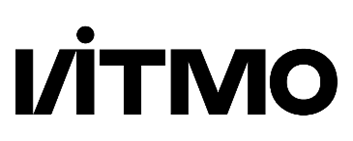
\includegraphics{logo}
\end{figure}
\vspace{-\baselineskip}


\begin{center}
	Федеральное государственное автономное образовательное \\
	учреждение высшего образования\\
	«Национальный исследовательский университет ИТМО»
\end{center}\par

\begin{center}
	\vspace{12pt}
	\Faculty
\end{center}\par

\vspace{\fill}
\begin{center}
	Лабораторная работа \LabNumber \\
	По дисципление: \LabSubject \\
	Тема: <<\LabName>> \\
	Вариант \Variant
\end{center}\par

\vspace{\fill}
\vbox{
	\hfill
	\vbox{
		\hbox{\textbf{Выполнил:} \StudentName}
		\hbox{\textbf{Группа:} \StudentGroup \\}
		\hbox{\textbf{Преподаватель:} \TeacherPosition \TeacherName}
	}
} 


\vspace{\fill}
\begin{center}
	Санкт-Петербург, \the\year{}
\end{center}\par

\newpage

	\twocolumn
\setcounter{figure}{4}
\begin{figure}[h]
	\centering
	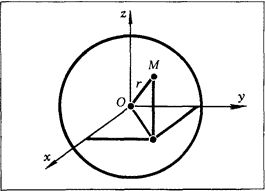
\includegraphics[width=1\linewidth]{circle}
	\caption{}
	\label{fig:circle}
\end{figure}
\vspace{-\baselineskip}

Уравнение сферы радиуса 50, центр которой сдвинут по оси $Ox$ на 30 единиц влево (именно такая сфера задана в примере 2), будет
$$(x - 30)^2 + y^2 + x^2 = 50^2.$$

Можно показать, что
$$x^2 + y^2 - \frac{1}{4}(x - 70)^2 = 0$$

\noindent - уравнение прямого кругового конуса, заданного на рисунке 4. При фиксированном $z = z_0$ оно принимает вид $x^2 + y^2 = \frac{(z - 70)^2}{4}$ и задает окружность - сечение конуса плоскостью $z = z_0$.

В данном примере мы быстро написали уравнение поверхностей в силу их простоты. Но, вообще говоря, уравнение поверхности, заданной на чертеже, надо выводить. В этом заключается задача первого этапа.

Итак, мы имеем следующую систему уравнений:
$$
\begin{cases}
	x^2 + y^2 - \frac{1}{4}(z - 70)^2 = 9, \\
	(x - 30)^2 + y^2 + z^2 = 50^2.
\end{cases}
$$

{\addfontfeatures{LetterSpace=20} Второй этап}. Вычтем из первого уравнения полученной системы второе. После простых преобразований получаем выражение
$$x = \frac{1}{48}z^2 - \frac{7}{12}z - \frac{75}{12}, \quad (*)$$
которое является уравнением фронтальной проекции линии пересечения конуса и сферы. Уравнение $(*)$ задает параболу, часть ее и изображена на рисунке 4.

Рассматривая теперь горизонтальную проекцию, из системы получим:
\begin{equation*}
	\begin{split}
		&x^2 + y^2 - \\
		&- \frac{1}{4}(\sqrt{50^2 - (x - 30)^2-y^2-70})^2 = 0
	\end{split}
\end{equation*}

Вот какую линию описывает это уравнение, сразу и не скажешь.

Чтобы построить обе кривые на проекциях, будет давать переменной $z$ в уравнение $(*)$ последовательно значения (например, с шагом $\delta z = 0,1$) в пределах $-42,5 \leq z \leq 46,5$ (эти пределы соответствуют крайним точкам $1`$ и $2`$ на фронтальной проекции, см. рис. 4). Для каждого значения переменной $z$ сначала вычислим по формуле $(*)$ значение переменной $x$, а затем (из уравнения сферы) найдем значение $y$ по формуле 
$$y = \pm \sqrt{50^2 - z^2 - (x - 30)^2}.$$
Указанный процесс вычислений легко осуществляется на ЭВМ. Таким образом, ЭВМ за короткий промежуток времени вычислит и напечатает координаты $x, y, z$ более $200$ точек линии пересечения. Теперь эти координаты надо в виде команд подать на чертежный автомат. Начинается третий этап. \\

\noindent\textbf{Чертежный автомат} \\
Существуют разные виды чертежных автоматов, которые по-разному стыкуются с вычислительными машинами. Современные чертежные автоматы (их часто называют \textit{графопостроителями}) типа Итекан (СССР), Бенсон (Франция; см. рис. 6), Дигиграф (Чехословакия) могут работать и от перфоленты, и от магнитной ленты, на которые выдает информацию вычислительная машина. Чертежный автомат может стыковаться с ЭВМ прямо через специальное переходное электронное устройство.

Большинство существующих чертежных автоматов выполнены с ли-

\newpage

\begin{table}[h]
	\begin{tabular}{lll}
		\hline
		\multicolumn{1}{c|}{Явление} & \multicolumn{1}{c|}{\begin{tabular}[c]{@{}c@{}}Момент \\ времени\end{tabular}} & \multicolumn{1}{c}{\rotatebox{90}{\parbox{1.2cm}{Фаза \\ затме\- \\ ния}}} \\ 
		\hline
		\multicolumn{1}{l|}{\multirow{2}{*}{Начало затмения}} & \multicolumn{1}{l|}{18 ноября} & \multirow{2}{*}{0,00} \\
		\multicolumn{1}{l|}{} & \multicolumn{1}{l|}{23 \textit{ч} 38 \textit{мин}} &  \\
		\multicolumn{1}{l|}{\multirow{3}{*}{Частные фазы}} & \multicolumn{1}{l|}{19 ноября} &  \\
		\multicolumn{1}{l|}{} & \multicolumn{1}{l|}{0 \quad 06} & 0,38 \\
		\multicolumn{1}{l|}{} & \multicolumn{1}{l|}{0 \quad 34} & 0,74 \\
		\multicolumn{1}{l|}{Начало полного затмения} & \multicolumn{1}{l|}{1 \quad 02} & 1,00 \\
		\multicolumn{1}{l|}{Наибольшая полная фаза} & \multicolumn{1}{l|}{1 \quad 23} & 1,07 \\
		\multicolumn{1}{l|}{Конец полного затмения} & \multicolumn{1}{l|}{1 \quad 44} & 1,00 \\
		\multicolumn{1}{l|}{\multirow{2}{*}{Частные фазы}} & \multicolumn{1}{l|}{2 \quad 12} & 0,74 \\ 
		\multicolumn{1}{l|}{Конец частного затмения} & \multicolumn{1}{l|}{3 \quad 08} & 0,38 \\
		\hline
	\end{tabular}
\end{table}
\end{document}